\documentclass[main.tex]{subfiles}
\begin{document}
\chapter{Functions and Relations}

\epigraph{They don't think it be like it is, but it do.}{Oscar Gamble}

\minitoc

\section{Introduction}

Sometimes in life you will have two (or more) things that are somehow related. Sometimes people make these relations for you. Sometimes you will be given two things and you have to come up with the relation. Our goal in this section is to give you the tools to solve these problems life throws at you. And remember, when life gets you down, just chuck some lemons back at him.

This chapter begins studying relations, then builds up to define functions.

\section{Relations}

% Relations are a formal way for us to map elements together in a similar fashion to functions. Unlike functions, however, a relation simply gives the \textit{relationship}. Sometimes you can construct a function that yields the relation. Other times, a function that would represent the relation would not be a function by definition.

Relations are a formal way for us to map elements together -- although this is not apparent at first. You may already be familiar with functions, \textit{mappings}, from high-school mathematics courses. We will build to functions using relations.

Relations simply give us a \textit{relation}ship between elements. We begin with a formal definition, then dive into relation classification.

\begin{defn}[Relation\index{Relation}]
	For sets \(A\) and \(B\), a relation \(R\) is any subset of the cross product of \(A\) and \(B\): \[R \subseteq \{(a,b) \in A \times B\}\]
	
	To specify that two elements are related under a relation \(R\) we say \(xRy\) which means \((x,y) \in R\)
\end{defn}

Here are a few examples:

\begin{example}
	An \textit{equality} relation \(\{(a,b) \mid a = b\} \subseteq \R \times \R\). This is a set of pairs where, for any given pair both elements in the pair are equal.
\end{example}

\begin{example}
	A \textit{less-than} relation \(\{(a,b) \mid a < b\} \subseteq \N \times \N\). This is a set of pairs where, for any given pair the first element is strictly less-than the second element.
\end{example}

\begin{example}
	The following is a relation, with \(A = \{2,4\}\) and \(B = \{6,8,10\}\): \(R = \{(x,y) \in A \times B \mid \frac{y}{x} \in \Z\} = \{(2,6), (2,10), (4,8)\}\)
\end{example}

\begin{rem}
	We will only consider relations of sets with themselves. We \textit{can} define relations between different sets, however this will make the following definitions significantly more challenging to define.
\end{rem}

\begin{defn}[Reflexive\index{Relation!Reflexive}]
	A relation \(R\) on a set \(A\) is reflexive if \[(\forall a \in A)[(a,a) \in R]\]
\end{defn}

\begin{defn}[Symmetric\index{Relation!Symmetric}]
	A relation \(R\) on a set \(A\) is symmetric if \[(\forall a,b \in A)[(a,b) \in R \Rightarrow (b,a) \in R]\]
\end{defn}

\begin{defn}[Transitive\index{Relation!Transitive}]
	A relation \(R\) on a set \(A\) is transitive if \[(\forall a,b,c \in A)[(a,b) \in R \land (b,c) \in R \Rightarrow (a,c) \in R]\]
\end{defn}

You will typically be asked to classify whether a relation satisfies the above three properties.

\exsol{
	Classify the following:
	
	\begin{center}
		\begin{tabular}{c|c|c|c}
			Relation & refl.\ & symm.\ & trans.\ \\ 
			\hline
			\(\{(1,1), (1,2), (2,1)\} \subseteq \{1,2\}^2\) & \(\lozenge\) & \(\lozenge\) & \(\lozenge\) \\
			\(\{(1,1), (1,2), (2,2)\} \subseteq \{1,2\}^2\) & \(\lozenge\) & \(\lozenge\) & \(\lozenge\) \\
			\(\{(x,y) \in \N \times \N \mid \frac{y}{x} \in \Z\}\) & \(\lozenge\) & \(\lozenge\) & \(\lozenge\) \\
			\(\{(x,y) \in \R^{\geq 1} \times \R^{\geq 1} \mid x < y^2\}\) & \(\lozenge\) & \(\lozenge\) & \(\lozenge\) \\
			\(\{(x,y) \in \R \times \R \mid (x=y) \lor (x=-y)\}\) & \(\lozenge\) & \(\lozenge\) & \(\lozenge\) \\
		\end{tabular}
	\end{center}
}{
	\(\blacklozenge\) indicates YES, \(\lozenge\) indicates NO
	
	\begin{center}
		\begin{tabular}{c|c|c|c}
			Relation & refl.\ & symm.\ & trans.\ \\ 
			\hline
			\(\{(1,1), (1,2), (2,1)\} \subseteq \{1,2\}^2\) & \(\lozenge\) & \(\blacklozenge\) & \(\lozenge\) \\
			\(\{(1,1), (1,2), (2,2)\} \subseteq \{1,2\}^2\) & \(\blacklozenge\) & \(\lozenge\) & \(\blacklozenge\) \\
			\(\{(x,y) \in \N \times \N \mid \frac{y}{x} \in \Z\}\) & \(\lozenge\) & \(\lozenge\) & \(\blacklozenge\) \\
			\(\{(x,y) \in \R^{\geq 1} \times \R^{\geq 1} \mid x < y^2\}\) & \(\lozenge\) & \(\lozenge\) & \(\lozenge\) \\
			\(\{(x,y) \in \R \times \R \mid (x=y) \lor (x=-y)\}\) & \(\blacklozenge\) & \(\blacklozenge\) & \(\blacklozenge\) \\
		\end{tabular}
	\end{center}
}

Oftentimes in computer science and mathematics we care about relations that satisfy all three properties. We even give these relations a fancy name, \textit{equality relation}.

\begin{defn}[Equivalence Relation\index{Relation!Equivalence Relation}]
	A relation that is reflexive, symmetric, and transitive
\end{defn}

The equivalence relation gives us a notion of \textit{equality}. If a relation \(R\) is an equivalence relation, then if \(xRy\) then we can think of \(x\) being ``equal'' to \(y\). The equals sign \(=\) gives us an equivalence relation on sets of numbers. In linear algebra, an isomorphism \(\cong\) is an equivalence relation on vector spaces. The mod operator \(\equiv\) gives us an equivalence relation on \(\Z\). As a real-life application, modular arithmetic is used in cryptography!

Here are some other cool definitions that probably will not be tested.

\begin{defn}[Antisymmetric\index{Relation!Antisymmetric}]
	A relation \(R\) on a set \(A\) is antisymmetric if \[(\forall a,b \in A)[(a,b) \in R \land (b,a) \in R \Rightarrow a = b]\]
\end{defn}

\begin{defn}[Composite of a Relation]
	If \(R \subseteq A \times B\) and \(S \subseteq B \times C\) are both relations, then the \textit{composite} of \(R\) and \(S\) is \[S \circ R = \{(a,c) \mid a \in A \land c \in C \land (b \in B \Rightarrow (a,b) \in R \land (b,c) \in S)\}\]
\end{defn}

\begin{defn}[Power of a Relation]
	If \(R \subseteq A \times A\) then for \(n \in \Z^+\) the \textit{power} \(R^n = R^{n-1} \circ R\) where \(R^1 = R\)
\end{defn}

\begin{thm}
	\label{relation-transitive-theorem}
	\(R \subseteq A \times A\) is transitive iff \(R^n \subseteq R\)
\end{thm}

The proof of this theorem is left as an exercise.

We have been discussing binary relations -- relations between two sets -- however we can define the notion of an \(n\)-ary relation. An \(n\)-ary relation is a subset of the cross product of \(n\) sets.

\begin{example}
	Here is a trinary (or \textit{ternary}) relation: \[R = \{(1,a,*), (2,a,+), (1,b,+)\} \subseteq \{1,2,3\} \times \{a,b,c,d\} \times \{*,+\}\]
\end{example}

The notions of reflexivity, symmetry, and transitivity also abstract to \(n\)-ary relations, as does an equivalence relation. This is outside the scope of this course.

\section{Functions}

Now that we understand relations, we can define a function.

\begin{defn}[Function\index{Function}]
	A relation \(R \subseteq C \times D\) that satisfies the following properties:
	\begin{enumerate}
		\item \((\forall c \in C)(\exists d \in D)[(c,d) \in R]\)
		\item \((\forall c \in C)(\forall d_1,d_2 \in D)[((c,d_1) \in R \land (c,d_2) \in R) \Rightarrow d_1 = d_2]\)
	\end{enumerate}
	
	If we recall the \textit{exists unique} symbol \(\exists!\), then we can combine the two properties above into one:
	\begin{enumerate}
		\item \((\forall c \in C)(\exists! d \in D)[(c,d) \in R]\)
	\end{enumerate}
\end{defn}

You may be familiar with the following less-formal definition.

\begin{defn}[Function\index{Function}]
	An explicit rule, or set of rules, that can be applied to a specified input to yield a specified output. There are two rules that all functions must follow:
	\begin{enumerate}
		\item Every input must be mapped to an output
		\item No input can map to more than one output
	\end{enumerate}
\end{defn}

Basically, functions give us a \textit{mapping} between sets -- a relation! For any relation \(R \subseteq C \times D\), we let the first set \(C\) be the function \textit{input} and the second set \(D\) be the function \textit{output}. If a pairing \((c,d) \in R\), then the function representing the relation \(R\) means that the function input \(c\) yields the output \(d\).

\exsol{
	Determine whether the following relations are functions.
	
	\begin{center}
		\begin{tabular}{c|c|c}
			Relation & is a func.\ & is not a func.\ \\ 
			\hline
			\(\{(x,y) \in \R \times \R^{\geq 0} \mid (x=y) \lor (x=-y)\}\) & \(\vartriangle\) & \(\vartriangle\) \\
			\(\{(x,y) \in \N \times \N \mid \frac{y}{x} \in \Z\}\) & \(\vartriangle\) & \(\vartriangle\) \\
			\(\{(x,y) \in \N \times \{1\} \mid \frac{x}{y} \in \Z\}\) & \(\vartriangle\) & \(\vartriangle\) \\
			\(\{(x,y) \in \N \times \{1\} \mid x < y\}\) & \(\vartriangle\) & \(\vartriangle\) \\
			\(\{(x,y) \in \N \times \{0\} \mid x \geq y\}\) & \(\vartriangle\) & \(\vartriangle\) \\
		\end{tabular}
	\end{center}
}{
	\(\blacktriangle\) indicates YES, \(\vartriangle\) indicates NO
	
	\begin{center}
		\begin{tabular}{c|c|c}
			Relation & is a func.\ & is not a func.\ \\ 
			\hline
			\(\{(x,y) \in \R \times \R^{\geq 0} \mid (x=y) \lor (x=-y)\}\) & \(\blacktriangle\) & \(\vartriangle\) \\
			\(\{(x,y) \in \N \times \N \mid \frac{y}{x} \in \Z\}\) & \(\vartriangle\) & \(\blacktriangle\) \\
			\(\{(x,y) \in \N \times \{1\} \mid \frac{x}{y} \in \Z\}\) & \(\blacktriangle\) & \(\vartriangle\) \\
			\(\{(x,y) \in \N \times \{1\} \mid x < y\}\) & \(\vartriangle\) & \(\blacktriangle\) \\
			\(\{(x,y) \in \N \times \{0\} \mid x \geq y\}\) & \(\blacktriangle\) & \(\vartriangle\) \\
		\end{tabular}
	\end{center}
}

Every function is a relation, but not every relation is a function. For any function, you can always write out the \((x,f(x))\) pairings -- this is by definition a relation. On the other hand, the above examples show that not every relation is a function.

The above relations are contrived examples. Typically we define functions on sets of numbers (we will restrict it to subsets of \(\R\)). We use the following notation to denote a function \(f\): \[f(x) = \text{some rules}\] and we pair the input/output sets as follows: \[f : D \rightarrow R\]

We might also notate functions by saying \(f : D \rightarrow R\) given by \(f : d \mapsto r\).

\begin{defn}[Domain\index{Function!Domain}]
	The set of inputs to a function
\end{defn}

\begin{defn}[Range\index{Function!Range}]
	The set containing all outputs to a function. This may also be called the \textit{co-domain}
\end{defn}

\begin{defn}[Image\index{Function!Image}]
	The set of all outputs to a function. This may be a subset of the function's range
\end{defn}

Let's look at some basic examples. First are some graphs of functions. Hopefully you learned how to plot 2-dimensional functions in previous math classes.

\begin{example}
	Here is a graph of the function \(f(x) = x\) where \(f : \R \rightarrow \R\)
	
	\begin{center}
		\begin{tikzpicture}
		% axes
		%\draw[latex-] (-4.5,0) -- (4.5,0) ;
		\draw[] (-3.5,0) -- (3.5,0) ;
		%\draw[latex-] (0,-4.5) -- (0,4.5) ;
		\draw[] (0,-3.5) -- (0,3.5) ;
		% ticks
		\foreach \x in  {-3,-2,-1,1,2,3} % x-axis
			\draw[shift={(\x,0)},color=black] (0pt,3pt) -- (0pt,-3pt);
		\foreach \x in  {-3,-2,-1,1,2,3} % y-axis
			\draw[shift={(0,\x)},color=black] (3pt,0pt) -- (-3pt,0pt);
		
		% func
		\draw[latex-,color=red] (-3,-3) -- (3,3) ;
		\draw[-latex,color=red] (-3,-3) -- (3,3) ;
		\end{tikzpicture}
	\end{center}
\end{example}

\begin{example}
	Here is a graph of the function \[f(x) = \begin{cases} x, & x > 2 \\ 1, & -2 \leq x \leq 2 \\ -x, & x < -2 \end{cases}\] where \(f : \R \rightarrow \R\)
	
	\begin{center}
		\begin{tikzpicture}
		% axes
		%\draw[latex-] (-4.5,0) -- (4.5,0) ;
		\draw[] (-3.5,0) -- (3.5,0) ;
		%\draw[latex-] (0,-4.5) -- (0,4.5) ;
		\draw[] (0,-1.5) -- (0,3.5) ;
		% ticks
		\foreach \x in  {-3,-2,-1,1,2,3} % x-axis
		\draw[shift={(\x,0)},color=black] (0pt,3pt) -- (0pt,-3pt);
		\foreach \x in  {-1,1,2,3} % y-axis
		\draw[shift={(0,\x)},color=black] (3pt,0pt) -- (-3pt,0pt);
		
		% func
		\draw[-latex,color=red] (2.05,2.05) -- (3,3) ;
		\draw[color=red] (-2,1) -- (2,1) ;
		\draw[latex-,color=red] (-3,3) -- (-2.05,2.05) ;
		\draw[color=red] (2,2) circle[radius=2pt];
		\fill[color=red] (2,1) circle[radius=2pt];
		\fill[color=red] (-2,1) circle[radius=2pt];
		\draw[color=red] (-2,2) circle[radius=2pt];
		\end{tikzpicture}
	\end{center}
\end{example}

Next we present examples of classifying whether a function is a function. To do this, recall the two requirements:
\begin{enumerate}
	\item Every input must be mapped to an output
	\item No input can map to more than one output
\end{enumerate}
You should check both of these requirements. For the first, recall that to dis-prove a universal statement you need a single counter-example. Thus, search the domain and make sure each input maps to an output

\exsol{
	Which of the following are functions? For the non-functions, change them such that they become functions.
	
	\begin{enumerate}[label=(\alph*)]
		\item \(a(x) = x\) where \(a : \Z \rightarrow \R\)
		\item \(b(x) = \sqrt{x}\) where \(b : \Z \rightarrow \R\)
		\item \(c(y) = \log_2(y)\) where \(c : \N \rightarrow \Z\)
		\item \(d(y) = y^2\) where \(d : \Z \rightarrow \N\)
		\item \(e(z) = \begin{cases} z + 1 & z \geq 0 \\ z - 1 & z \leq 0 \end{cases}\) where \(e : \R \rightarrow \Z\)
	\end{enumerate}
}{
	\begin{enumerate}[label=(\alph*)]
		\item Function
		\item Not a function -- \(b\) does not work for any negative input, however the domain is set to \(\Z\). Simply change the domain to \(\N\)
		\item Not a function -- \(c(3) \not\in \Z\) thus not every input is mapped to an output. Change the co-domain to positive real numbers
		\item Function
		\item Not a function -- (1) the input \(z = 0\) has two different outputs \(e(0) = 1\) and \(e(0) = -1\), (2) any real number that is not an integer does not have a mapping in the range (ex: \(e(1.5) = 1.5 + 1 = 2.5 \not\in \Z\)). Change one of the cases to not include 0, then either change the range to \(\R\) or change the domain to \(\Z\)
	\end{enumerate}
}

There exist 3 properties that any function can have.

\begin{defn}[Injection (One-to-One)\index{Function!Injective}]
	A function where each co-domain (range) value is mapped to by at most one value in the domain. In other words, each value in the range has either 0 or 1 pointers from the domain. Formally, \(f : D \mapsto R\) is injective iff \[(\forall x_1,x_2 \in D)[f(x_1) = f(x_2) \Rightarrow x_1 = x_2]\]
	The horizontal line test can be used to see if a function is injective
\end{defn}

\begin{defn}[Surjection (Onto)\index{Function!Surjective}]
	A function where each co-domain (range) value is mapped to by at least one value in the domain. In other words, there are no un-mapped values in the range. Formally, \(f : D \mapsto R\) is surjective iff \[(\forall y \in R)(\exists x \in D)[y = f(x)]\]
\end{defn}

\begin{defn}[Bijection (One-to-One Correspondence)\index{Function!Bijective}]
	A function that is both an injection and a surjection. Every input is mapped to exactly one unique output
\end{defn}

You should know how to identify these properties in functions. To test injectivity, perform the horizontal line test -- run a horizontal line vertically along the graph of the function; the function is injective if the horizontal line never touches more than one point. To test surjectivity, ask yourself if you can ``get to'' every output element. To be bijective, you must both be injective and surjective. A function can be neither injective nor surjective, but still be a function.

We can represent a function by drawing ovals representing the domain and range, drawing points in each oval representing the elements in each set, and drawing arrows between the points representing the function mapping. In this way, we present a visual guide to the above definitions.

\begin{figure}[H]
	\centering
	\begin{tabular}{ c l | l }
		& Injection & Not Injection \\
		\rotatebox[origin=l]{90}{Surjection} &%
		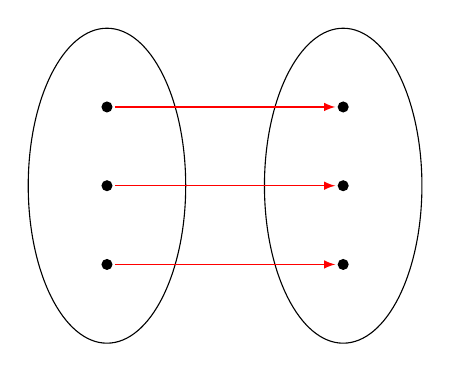
\begin{tikzpicture}
		\draw (0,0) ellipse (1cm and 2cm);
		\draw (3,0) ellipse (1cm and 2cm);
		\fill (0,1) circle[radius=2pt];
		\fill (0,0) circle[radius=2pt];
		\fill (0,-1) circle[radius=2pt];
		\fill (3,1) circle[radius=2pt];
		\fill (3,0) circle[radius=2pt];
		\fill (3,-1) circle[radius=2pt];
		\draw[-latex,color=red] (0.1,1) -- (2.9,1) ;
		\draw[-latex,color=red] (0.1,0) -- (2.9,0) ;
		\draw[-latex,color=red] (0.1,-1) -- (2.9,-1) ;
		\end{tikzpicture}%
		&%
		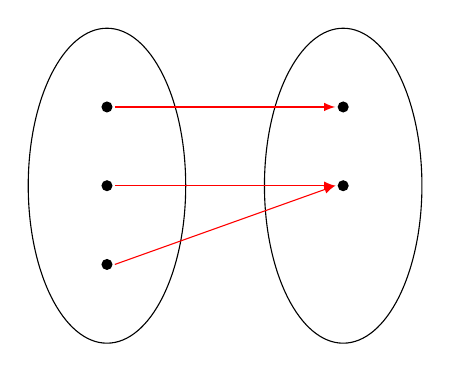
\begin{tikzpicture}
		\draw (0,0) ellipse (1cm and 2cm);
		\draw (3,0) ellipse (1cm and 2cm);
		\fill (0,1) circle[radius=2pt];
		\fill (0,0) circle[radius=2pt];
		\fill (0,-1) circle[radius=2pt];
		\fill (3,1) circle[radius=2pt];
		\fill (3,0) circle[radius=2pt];
		\draw[-latex,color=red] (0.1,1) -- (2.9,1) ;
		\draw[-latex,color=red] (0.1,0) -- (2.9,0) ;
		\draw[-latex,color=red] (0.1,-1) -- (2.9,0) ;
		\end{tikzpicture}%
		\\
		\midrule
		\rotatebox[origin=l]{90}{Not Surjection} &%
		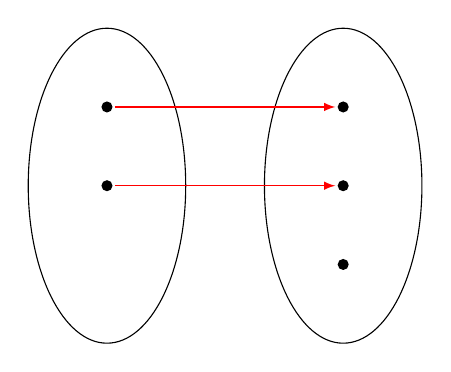
\begin{tikzpicture}
		\draw (0,0) ellipse (1cm and 2cm);
		\draw (3,0) ellipse (1cm and 2cm);
		\fill (0,1) circle[radius=2pt];
		\fill (0,0) circle[radius=2pt];
		\fill (3,1) circle[radius=2pt];
		\fill (3,0) circle[radius=2pt];
		\fill (3,-1) circle[radius=2pt];
		\draw[-latex,color=red] (0.1,1) -- (2.9,1) ;
		\draw[-latex,color=red] (0.1,0) -- (2.9,0) ;
		\end{tikzpicture}%
		&%
		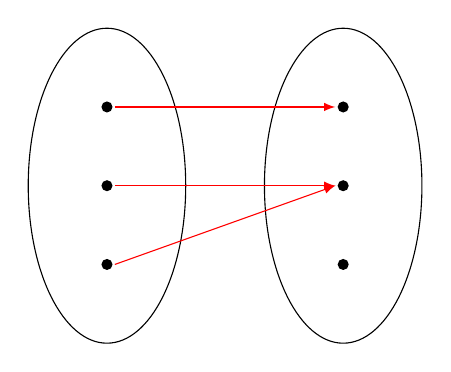
\begin{tikzpicture}
		\draw (0,0) ellipse (1cm and 2cm);
		\draw (3,0) ellipse (1cm and 2cm);
		\fill (0,1) circle[radius=2pt];
		\fill (0,0) circle[radius=2pt];
		\fill (0,-1) circle[radius=2pt];
		\fill (3,1) circle[radius=2pt];
		\fill (3,0) circle[radius=2pt];
		\fill (3,-1) circle[radius=2pt];
		\draw[-latex,color=red] (0.1,1) -- (2.9,1) ;
		\draw[-latex,color=red] (0.1,0) -- (2.9,0) ;
		\draw[-latex,color=red] (0.1,-1) -- (2.9,0) ;
		\end{tikzpicture}%
		\\
	\end{tabular}
	\caption{Injection and Surjection}
\end{figure}

\exsol{
	Classify the following:
	
	\begin{center}
	\begin{tabular}{lc|c|c|c|c}
		& & func.\ & inj.\ & surj.\ & bij.\ \\ 
		\hline
		\(f(x) = x\) & \(f : \N \rightarrow \Z\) & \(\lozenge\) & \(\lozenge\) & \(\lozenge\) & \(\lozenge\) \\
		\(g(x) = x\) & \(g : \Z \rightarrow \Z\) & \(\lozenge\) & \(\lozenge\) & \(\lozenge\) & \(\lozenge\) \\
		\(h(x) = x^2\) & \(h : \R \rightarrow \N\) & \(\lozenge\) & \(\lozenge\) & \(\lozenge\) & \(\lozenge\) \\
		\(i(x) = \floor{x^2}\) & \(i : \R \rightarrow \N\) & \(\lozenge\) & \(\lozenge\) & \(\lozenge\) & \(\lozenge\) \\
		\(j(x) = x^3-x\) & \(j : \Z \rightarrow \R\) & \(\lozenge\) & \(\lozenge\) & \(\lozenge\) & \(\lozenge\) \\
	\end{tabular}
	\end{center}
}{
	\(\blacklozenge\) indicates YES, \(\lozenge\) indicates NO
	
	\begin{center}
	\begin{tabular}{lc|c|c|c|c}
		& & func.\ & inj.\ & surj.\ & bij.\ \\ 
		\hline
		\(f(x) = x\) & \(f : \N \rightarrow \Z\) & \(\blacklozenge\) & \(\blacklozenge\) & \(\lozenge\) & \(\lozenge\) \\
		\(g(x) = x\) & \(g : \Z \rightarrow \Z\) & \(\blacklozenge\) & \(\blacklozenge\) & \(\blacklozenge\) & \(\blacklozenge\) \\
		\(h(x) = x^2\) & \(h : \R \rightarrow \N\) & \(\lozenge\) & \(\lozenge\) & \(\lozenge\) & \(\lozenge\) \\
		\(i(x) = \floor{x^2}\) & \(i : \R \rightarrow \N\) & \(\blacklozenge\) & \(\lozenge\) & \(\blacklozenge\) & \(\lozenge\) \\
		\(j(x) = x^3-x\) & \(j : \Z \rightarrow \R\) & \(\blacklozenge\) & \(\lozenge\) & \(\lozenge\) & \(\lozenge\) \\
	\end{tabular}
	\end{center}
}

Hash tables are an important application of functions in computer science. A hash table is a data structure; it is a fancy array. A hash table has an internal array, and a hash function. This hash function maps table elements (some set of objects) to indices (\(\N\)). The modulus of the hash function output, with respect to the table size, is taken as the input object's key. This is where the object is stored in the table. Ideally, you want your hash function to be an injection on the set of indices.

\begin{thm}
	A bijection \(f : A \rightarrow B\) is invertible, and the inverse, denoted \(f^{-1} : B \rightarrow A\), is also a bijection.
\end{thm}

\begin{proof}
	First note that \textit{inverse} simply means that \(f^{-1}(f(a)) = a\). With this in mind, then we note that \(f^{-1}(b) = a\) such that \(f(a) = b\). Then since \(f\) is a bijection, \(b\) is the one-and-only output that \(a\) maps to. Then \(a\) is the one-and-only output that \(b\) maps to in \(f^{-1}\). So it is a bijection.
	
	We can show this more formally by showing \(f^{-1}\) is an injection and a surjection.
	
	\textbf{1-1}: Let \(f^{-1}(b_1) = f^{-1}(b_2)\), then \(f(f^{-1}(b_1)) = f(f^{-1}(b_2)) \Rightarrow b_1 = b_2\).
	
	\textbf{onto}: Let \(f^{-1}(b) = a\), then \(b = f(a)\) which exists because \(f\) is a bijection.
	
	You should prove on your own that indeed \(f^{-1}\) is a function!
\end{proof}

\begin{thm}
	The composition of bijective functions is a bijection.
\end{thm}

\begin{proof}
	Let \(f,g\) be the bijections \(f : A \mapsto B\) and \(g : B \mapsto C\). Then by the previous theorem \(f,g\) have inverses which are also bijections.
	
	Define \(h : A \mapsto C\) given by \(h : a \mapsto g(f(a)) = (g \circ f)(a)\).
	
	\textbf{1-1}: Let \(h(a_1) = h(a_2)\), then \(g(f(a_1)) = g(f(a_2)) \Rightarrow f^{-1}(g^{-1}(g(f(a_1)))) = f^{-1}(g^{-1}(g(f(a_2)))) \Rightarrow a_1 = a_2\)
	
	\textbf{onto}: Let \(h(a) = c\), then \(g(f(a)) = c\) so \(a = f^{-1}(g^{-1}(c))\) exists.
\end{proof}

\section{Sequences}

Sequences make up an interesting sub-part of functions. In calculus, we build up continuous functions as limits of sequences. This is discrete mathematics, however, so sequences will be of more interest to us.

\begin{defn}[Sequence\index{Sequence}]
	An ordered list of numbers, each one associated with a specific \textit{position} (index)
\end{defn}

For the purposes of this class, you can think of a sequence as a mapping between the natural numbers and the associated index in the sequence. Sometimes you can express a sequence as a closed-form function, and sometimes a sequence can have multiple interpretations. Let's look at a few examples to get the notation down.

\begin{example}
	The following three notations describe the same sequence:
	
	\begin{enumerate}[label=(\alph*)]
		\item \(1, 3, 7, 15, 31, \dots\)
		\item \(a_n = \begin{cases} 1 &,\ n = 1 \\ 2a_{n-1} + 1 &,\ n > 1 \end{cases},\ n \in \Z^+\)
		\item \(f(n) = 2^n - 1\) where \(f : \Z^+ \mapsto \Z^+\)
	\end{enumerate}
\end{example}

We have explicit names for the notation types in the previous example.

\begin{defn}[General Form\index{Sequence!General Form}]
	A written list of the elements of a sequence, in order, typically with \(\dots\) at the end (and at the beginning, if your sequence elements start in the middle -- typically this does not happen). Sometimes mathematicians put curly braces \(\{\}\) around their general-form sequences -- try not to get this confused with a set! Other times mathematicians will give you a rule, written in plain English, for generating sequence terms
\end{defn}

\begin{defn}[Recursive Form\index{Sequence!Recursive Form}]
	An explicit formula that depends on previous elements in the sequence, and necessarily has one or more base cases. Typically this is expressed as \[x_n = \begin{cases} \text{base case(s)} &, n \in \{\text{some set}\} \\ \text{some formula dependent on } n &, n \not\in \{\text{the previous set}\} \end{cases}\]
\end{defn}

\begin{defn}[Closed Form\index{Sequence!Closed Form}]
	An explicit formula to generate a specific term in a sequence. This formula is solely dependent on a given index. Typically this is expressed as \[y_k = \text{some formula dependent on } k\]
\end{defn}

\begin{rem}
	Sequence numbers do not need to be in any particular order, nor do they necessarily have to fit some sort of function. Sequences elements can also be any sort of number (we will restrict to \(\R\)).
\end{rem}

\begin{example}
	Some sequences:
	\[1, 0, -1, 0, 1, 0, -1, 0, \dots\]
	\[8, 6, 4, 2, 8, 6, 4, 2, 8, \dots\]
	\[0, 0.5, 0.333, 0.25, 0.2, 0.125, \dots\]
\end{example}

Sometimes we will ask you to generate terms of a sequence. This is a relatively straightforward task so long as you avoid simple arithmetic errors. 

\exsol{
	Generate the first 7 terms of the following sequences:
	
	\begin{enumerate}[label=(\alph*)]
		\item The \(n\)th term is its index tripled (start your indices at 0)
		\item \(f_k = \begin{cases} 1 &, k = 1,2 \\ f_{k-1} + f_{k-2} &, k \geq 3 \end{cases}\)
		\item \(l_1 = l_2 = l_3 = 1\) and \(l_i = l_{i-1} + l_{i-2} + l_{i-3}\)
	\end{enumerate}
}{
	We will use \(\{\}\) notation here:
	
	\begin{enumerate}[label=(\alph*)]
		\item A simple rule (one that we could express in closed form) -- \(\{0, 3, 6, 9, 12, 15, 18, \dots\}\)
		\item This is the Fibonacci sequence -- \(\{1, 1, 2, 3, 5, 8, 13, \dots\}\)
		\item In this case, the index is implied to be \(\in \Z^+\) -- \(\{1, 1, 1, 3, 5, 9, 17, \dots\}\)
	\end{enumerate}
}

Other times we will ask you to find a closed form for a sequence given in general or recursive form. Typically we ask this about general forms, however occasionally you will see a recursive form. This task is akin to pattern-matching and sometimes requires much more critical thinking. Sometimes sequences can have multiple answers -- any correct answer suffices. Answers that are unreasonable -- i.e.\ answers that only fit the provided sequence digits -- will receive a good chuckle along with zero marks.

\exsol{
	Find closed-forms for the following sequences:
	
	\begin{enumerate}[label=(\alph*)]
		\item \(\{1, 4, 9, 16, 25, \dots\}\)
		\item \(\{3, 6, 9, 12, 15, \dots\}\)
		\item \(\{1, 4, 9, 6, 5, 6, 9, \dots\}\)
		\item \(\{1, 1, 1, 2, 2, 2, 2, 2, 3, 3, 3, 3, 3, 3, 3, 4, \dots\}\)
		\item \(\{2, 5, 8, 0, 3, 6, 9, \dots\}\)
	\end{enumerate}
}{
	We attempt to explain the patterns that led us to the solutions:
	
	\begin{enumerate}[label=(\alph*)]
		\item The pattern here is squares. Each sequence number is the square of its index
		\item \(f(n) = 3(n+1)\) where \(f : \N \rightarrow \Z\)
		\item Hopefully you still had the first sequence in mind -- squares modulo 10
		\item Notice a pattern with the indices -- specifically look at the index where there is a switch. Index 1 starts the 1s, index 4 starts the 2s, index 9 starts the 3s, index 16 starts the 4s. What is the relationship between these numbers? Take the square root of the index. Then realize that square roots maintain inequalities -- \(1 = \sqrt{1} < \{\sqrt{2}, \sqrt{3}\} < \sqrt{4} = 2\), so look towards floors and ceilings to yield integers. Thus, \(f(n) = \floor{\sqrt{n}}\) where \(f : \Z^+ \rightarrow \Z^+\)
		\item This one can have multiple answers. One solution: \(f(n) = 3n-1 \Mod{11}\) (taking least positive remainder) where \(f : \Z^+ \rightarrow \Z^+\). Typically if you see a somewhat circular sequence, especially if there is a zero, then consider applying a modulus. Start at the zero and look forward until the sequence reverts. In this case, we have \(0,3,6,9\) which is simply \(f(n) = 3n\). Then play around with the start point and the modulus
	\end{enumerate}
}

Finding a closed-form function that matches a sequence is difficult. It requires a deep understanding of how all mathematical operators work, and requires a knack for finding patterns. There are multiple methods for estimating functions, including polynomial interpolation, piece-wise functions, floor-ceiling interpolation, and least-squares. These methods usually yield a result significantly more complicated than finding a simpler function. However, there are merits to using these methods as a starting-point.

\subsection{Series}

You may remember series from a calculus course. Series are closely related to sequences.

\begin{defn}[Series\index{Series}]
	The sum of all terms in a sequence
\end{defn}

\begin{example}
	The Geometric Series (\(r \neq 1\)) \[a + ar + ar^2 + \cdots ar^{n-1} = \sum_{i=0}^{n-1} ar^i\]
	which has the solution \[= a(\frac{1-r^n}{1-r})\]
\end{example}

Typically we try to understand the limiting behavior of infinite series. There are a number of tests you can use to study this behavior, however this topic is typically taught in Calculus II classes. We will thus omit this topic here, however we do recommend at least understanding the idea behind limits. We will come back to infinite objects when we discuss countability in chapter \ref{chapter:countability}.

\exsol{
	Determine whether the series \(\sum_{i=1}^{\infty}\frac{1}{3^{i-1}}\) converges or diverges.
}{
	From the geometric series formula above, \(\sum_{i=1}^{n} \frac{1}{3^{i-1}} = \sum_{i=0}^{n-1} \frac{1}{3^i} = \sum_{i=0}^{n-1} \frac{1}{3}^i = \frac{1-\frac{1}{3}^n}{1 - \frac{1}{3}} = \frac{3}{2}(1-\frac{1}{3^n})\). Then we can take the limit as \(n \rightarrow \infty\), which \(= \frac{3}{2}(1 - 0) = \frac{3}{2}\)
}

\section{Summary}

\begin{itemize}
	\item Relations give us a formal way to write out a mathematical relationship between elements in sets.
	\item Functions are a special kind of binary relation that satisfy \((\forall c \in C)(\exists! d \in D)[(c,d) \in R]\). A function \(f : C \mapsto D\) is then described by the input/output pairs \((c,d) \in R\).
	\item Sequences have three forms: general, recursive, and closed.
\end{itemize}

\section{Practice}

\begin{enumerate}
	\item Write out the \textit{greater than} relation \(R \subseteq \{1,2,3\} \times \{-1,1,3,5\}\)
	\item Classify the following relations as reflexive, symmetric, and/or transitive:
	\begin{enumerate}
		\item \(\{(x,y) \in \N \times \N \mid x \leq \sqrt{y}\}\)
		\item \(\{(x,y) \in \N \times \N \mid x \equiv y^2 \Mod{4}\}\)
		\item \(\{(x,y) \in \N \times \N \mid \sqrt{x} \leq y\}\)
	\end{enumerate}
	\item Prove Theorem \ref{relation-transitive-theorem}.
	\item Determine whether the following relations are functions:
	\begin{enumerate}
		\item \(\{(x,y) \in \Z^- \times \Z^+ \mid x < y\}\)
		\item \(\{(x,y) \in \Z^+ \times \Z^- \mid x < y\}\)
		\item \(\{(x,y) \in \R   \times \R   \mid y = x + 2\}\)
	\end{enumerate}
	\item Why is the relation \(\{(x,y) \in \Z \times \Z \mid x \equiv y \Mod{m}\}\) \textbf{not} a function?
	\item Determine whether the following are functions. If they are, then classify them as injective, surjective, and/or bijective.
	\begin{enumerate}
		\item \(f : \Z \rightarrow \Z\) given by \(f : z \mapsto \% 37\)
		\item \(f : \Q \rightarrow \Q\) given by \(f : q \mapsto \sqrt{q}\)
		\item \(f : \R \rightarrow \Z\) given by \(f : x \mapsto \floor{x}\)
	\end{enumerate}
	\item Suppose a function \(f : X \rightarrow Y\) is injective and \(h : X \rightarrow X\) is bijective. Is the function \(g : X \rightarrow Y\) given by \(g(x) = f(h(x))\) also injective? What if \(h\) is only surjective? What if \(h\) is only injective? % is this a stupid question?
	\item Find closed-forms, or simple rules, that describe the following sequences:
	\begin{enumerate}
		\item \(\{-3,-1,1,3,5,\cdots\}\) % odds, shifted back
		\item \(\{-1, 1, 7, 25, 79, \cdots\}\) % 3^i - 2
		\item \(\{2,3,5,0,4,\cdots\}\) % primes mod 7
	\end{enumerate}
	% todo
\end{enumerate}

\end{document}

